\documentclass{beamer}                             % presentation
% \documentclass[draft]{beamer}                    % improves compile time
% 4' x 3' poster (48" x 36")
\usepackage[orientation=landscape,size=custom,width=121.92,height=91.44,
scale=1.4,debug]{beamerposter}
% replace default beamer blocks for more customization of outlines
% https://tex.stackexchange.com/questions/11484/how-to-draw-a-frame-box-around-an-arbitrary-large-piece-of-text-figures-whatever
\usepackage{tcolorbox}
\usepackage[utf8]{inputenc}                        % utf8
\usepackage[T1]{fontenc}                           % fix font encoding
\usepackage{lmodern}                               % arbitrarily large font
\usepackage[english]{babel}                        % language
\usepackage{geometry, hyperref, fancyhdr, algorithm}
\usepackage{amsmath, amssymb, amsthm}              % ams mathematical packages
\usepackage{physics, mathtools, bm}                % extra math packages
\usepackage{graphicx, subcaption, wrapfig}         % images
\usepackage{svg}                                   % svg images
\usepackage{fvextra, textcomp, CJKutf8}            % misc. text formatting
\usepackage[autostyle, english=american]{csquotes} % quotes
\usepackage{tikz, pgfplots}                        % plots and graphs
\usepackage[noend]{algpseudocode}                  % algorithm psuedocode
\usepackage[cache=true]{minted}                    % source code
\usepackage[style=ieee]{biblatex}                  % bibliography

\addbibresource{refs.bib}
\usetikzlibrary{positioning}                       % advanced positioning
\pgfplotsset{compat=newest}                        % version of pgfplots
\usepgfplotslibrary{fillbetween}

\graphicspath{{./figs/}}

\newcommand{\blocktitle}[1]{{\Large \textbf{#1}}}
\renewcommand\mathfamilydefault{cmr}

\newcommand{\GeV}{\,{\rm GeV}}

%%% colors

\definecolor{lightblue}{HTML}{a1b4c7}
\definecolor{orange}{HTML}{ea8810}
\definecolor{silver}{HTML}{b0aba8}
\definecolor{rust}{HTML}{b8420f}
\definecolor{seagreen}{HTML}{23553c}

\colorlet{lightsilver}{silver!20!white}
\colorlet{darkorange}{orange!85!black}
\colorlet{darksilver}{silver!85!black}
\colorlet{darklightblue}{lightblue!75!black}
\colorlet{darkrust}{rust!85!black}
\colorlet{darkseagreen}{seagreen!85!black}

\colorlet{zeroborder}{darksilver}
\colorlet{zerocolor}{lightsilver}
\colorlet{nnzborder}{darksilver}
\colorlet{nnzcolor}{silver}

\colorlet{colborder}{black}
\colorlet{targetcolor}{orange}
\colorlet{selcolor}{seagreen}
\colorlet{candcolor}{lightblue}
\hypersetup{
  colorlinks=true,
  linkcolor=darkrust,
  citecolor=darkseagreen,
  urlcolor=seagreen
}

\pgfplotsset{
  every axis plot/.append style={line width=4},
  every mark/.append style={mark size=32},
}

%%% beamer settings

\usetheme{Pittsburgh}

\setbeamertemplate{navigation symbols}{}
\setbeamercolor{title}{fg=darkrust}
\setbeamercolor{frametitle}{fg=darkrust}
\setbeamercolor{bibliography entry author}{fg=darkrust}
\setbeamercolor{bibliography entry institute}{fg=darkrust}
\setbeamercolor{bibliography entry note}{fg=darkrust}

\renewcommand*{\bibfont}{\small}

\tcbset{
  % skin=enhanced,
  colframe=darkrust,
  colback=white,
  % coltitle=black,
  % colbacktitle=white,
  % fonttitle={\Large\bfseries},
  % titlerule=0mm,
  % titlerule style={draw=none, line width=0mm},
}

% margin
\setbeamersize{text margin left=1.27cm, text margin right=1.27cm}

% title page
\title[]{\Huge Stochastic Gravitational Wave Background Detection through \\ NANOGrav 15-year Data Set in the View of Massive Gravity}
\author[Choi]{\LARGE \textbf{Chris Choi$\,^1$}, Jacob Magallanes$\,^1$, Murman Gurgenidze$\,^{1,2}$, and Tina Kahniashvili$\,^{1,2,3}$}
\institute[]{\large $\,^1$Carnegie Mellon University, $\,^2$Ilia State University, $\,^3$Abastumani Astrophysical Observatory}
\date[]{}
\subject{Physics}

\begin{document}
\begin{frame}[t]
\vspace{-1em}
\titlepage

% CMU logo in top left
\begin{tikzpicture}[overlay,remember picture]
  \node[below right=1cm and 3cm] at (current page.north west) {
      \includesvg[width=0.15\columnwidth]{CMU_stacked}
  };
\end{tikzpicture}

% QR code in top right
\begin{tikzpicture}[overlay,remember picture]
  \node[below left=1.27cm and 1.27cm] at (current page.north east) {
      \includesvg[width=0.11\columnwidth]{qr-code}
    };
\end{tikzpicture}

% remove gap
\vspace{-6cm}

\begin{center}
  \textcolor{darksilver}{\rule{\textwidth}{2mm}}
\end{center}

\begin{columns}[T]

%%% column 1

\begin{column}{0.30\textwidth}
  \begin{tcolorbox}
    \blocktitle{Abstract}
    \begin{itemize}
        \item Convincing evidence of a stochastic gravitational wave background (SGWB) has been found by the NANOGrav 15-year data set (NG15). 
        \item We evaluate the possibility of its source being from the early universe through massive tensor perturbations induced by parametric resonance. 
        \item We find values of the graviton mass, mass cutoff time, and Hubble rate of inflation that amplify the energy spectra of primordial GWs to reproduce NG15 within 1-3$\sigma$. 
        \item However, it is difficult to obey the BBN and CMB bound without introducing a suppression mechanism or making the graviton mass cutoff time too deep into the matter dominated era.
    \end{itemize}
  \end{tcolorbox}

  \begin{tcolorbox}
    \blocktitle{Background}
    \begin{itemize}
        \item First detection of SGWB by NANOGrav collaboration in 2023 \cite{Agazie:2023}
        \item Most popular explanation is astrophysical: inspiraling supermassive black hole binaries (SMBHBs) emitting low-frequency GWs \cite{Burke-Spolaor:2018bvk}.
        \item More exotic explanations lie in cosmological sources: cosmic strings, domain walls, first-order phase transitions, primordial magnetic fields, primordial GWs, scalar-induced GWs, etc \cite{Afzal:2023}.  
        \item We explore the explanation of primordial GWs generated during inflation, amplified by massive gravity.
    \end{itemize}
    \begin{figure}[t]
      \centering
      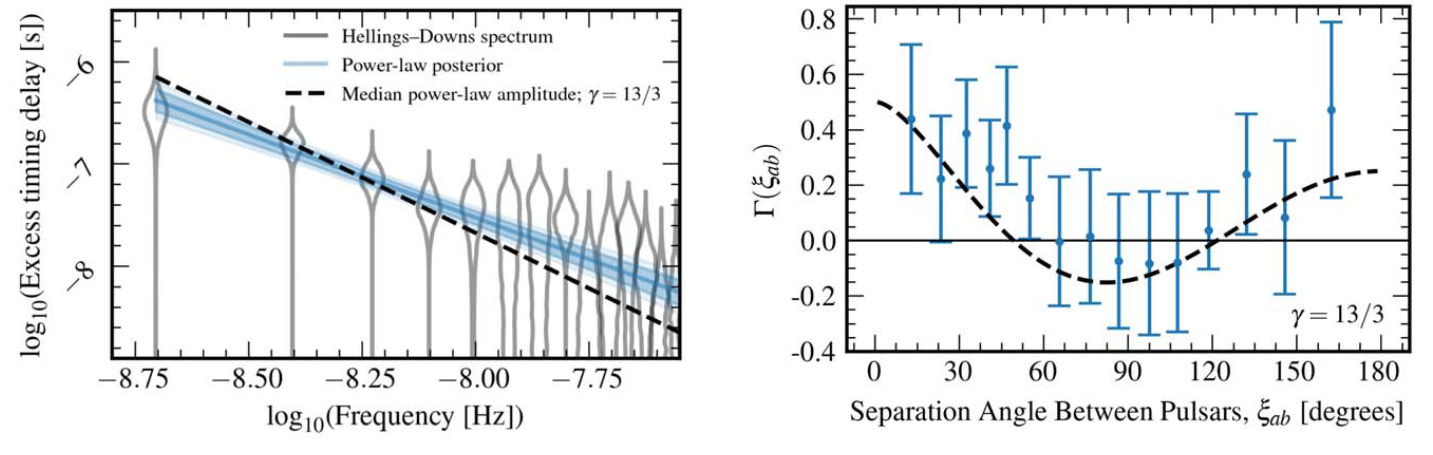
\includegraphics[width=\linewidth]{ng15.png}  
      \label{fig:ng15}
    \end{figure}
  \end{tcolorbox}

  \begin{tcolorbox}
    \blocktitle{Massive Gravity}
    \vspace{0.25\baselineskip}
    \begin{columns}
      \hfill
      \begin{column}{0.5\textwidth}
      \begin{itemize}
          \item  We consider model of MTMG \cite{DeFelice:2015hla} where graviton mass $M_{\text{GW}}$ is step-function of time \cite{Fujita:2018ehq}
          \item Equation of motion for the two tensor modes:
      \end{itemize} 
      $$\bar{h}_k'' + \left(k^2 + a^2 M_\text{GW}^2 - \frac{a''}{a}\right)\bar{h}_k = 0 $$  
    \begin{itemize}
        \item Scale factor $a$ and graviton mass are defined as follows:
    \end{itemize}
        $$a(\tau) = 
    \begin{cases}
        -1/(H_{\inf}\tau) & \tau < \tau_r \\
        a_r \tau/\tau_r & \tau > \tau_r \\
   \end{cases} $$
    $$M_\text{GW}(\tau) = 
    \begin{cases}
        m & \tau < \tau_m \\
        0 & \tau > \tau_m
   \end{cases}$$
      \end{column}
      \begin{column}{0.48\textwidth}
        \begin{figure}[t]
          \centering
          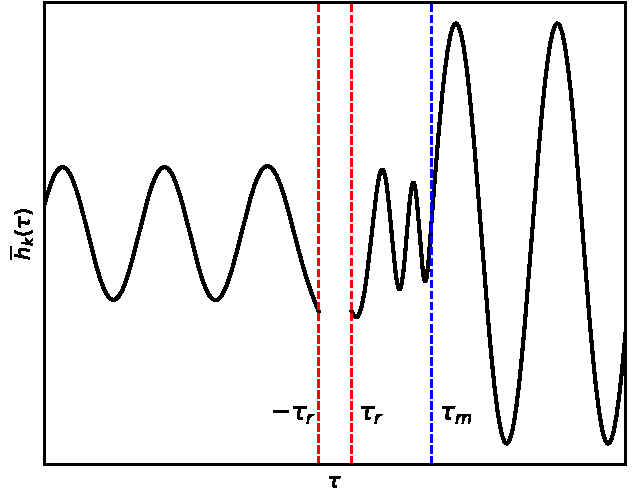
\includegraphics[width=\linewidth]{fig1.pdf} 
          \label{fig:mode}
        \end{figure}
      \end{column}
    \end{columns}
  \end{tcolorbox}
\end{column}

\begin{column}{0.01\textwidth}
  \begin{center}
    \textcolor{darksilver}{\rule[-1cm]{1mm}{0.8\textheight}}
  \end{center}
\end{column}

%%% column 2

\begin{column}{0.30\textwidth}
  \begin{tcolorbox}
    \blocktitle{Energy Density of GWs}
    
    \begin{itemize}
        \item The present-day energy densities of GWs help us look at how primordial GWs are influenced by deviations from GR
        \item Energy density is defined as 
    \end{itemize}
    $$\Omega_\text{GW} = \frac{1}{\rho_c}\frac{d \rho_\text{GW}} {d \log{k}}$$

    \begin{itemize}
        \item In massive gravity, $\Omega_{\text{GW}}$ is blue tilted / amplified:
    \end{itemize}
    $$\Omega_{\text{GW},0}(f) = \frac{\pi^2f^2}{3a_0^2 H_0^2}\frac{\tau_m}{\tau_r}(k\tau_r)^{3-2\nu}\mathcal{P}_{\text{GR}}(k)$$
    \begin{itemize}
        \item $\mathcal{P}_{\text{GR}}(k)$ is defined in our paper \cite{Choi:2023tun} in Eq.\ 14.
        \item $\nu$ in the exponent is defined as 
    \end{itemize}
    $$\nu = \sqrt{\frac{9}{4} - \frac{m^2}{H_{\inf}^2}}$$
     \begin{figure}[t]
          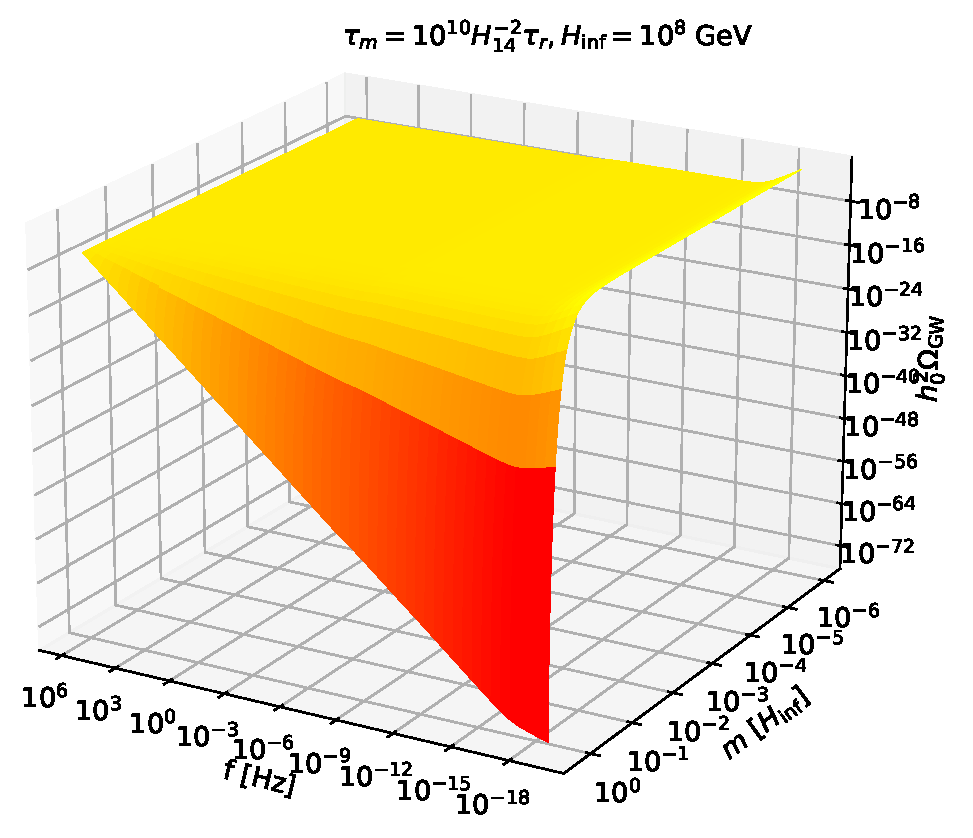
\includegraphics[width=.32\linewidth]{fig4a.pdf} 
          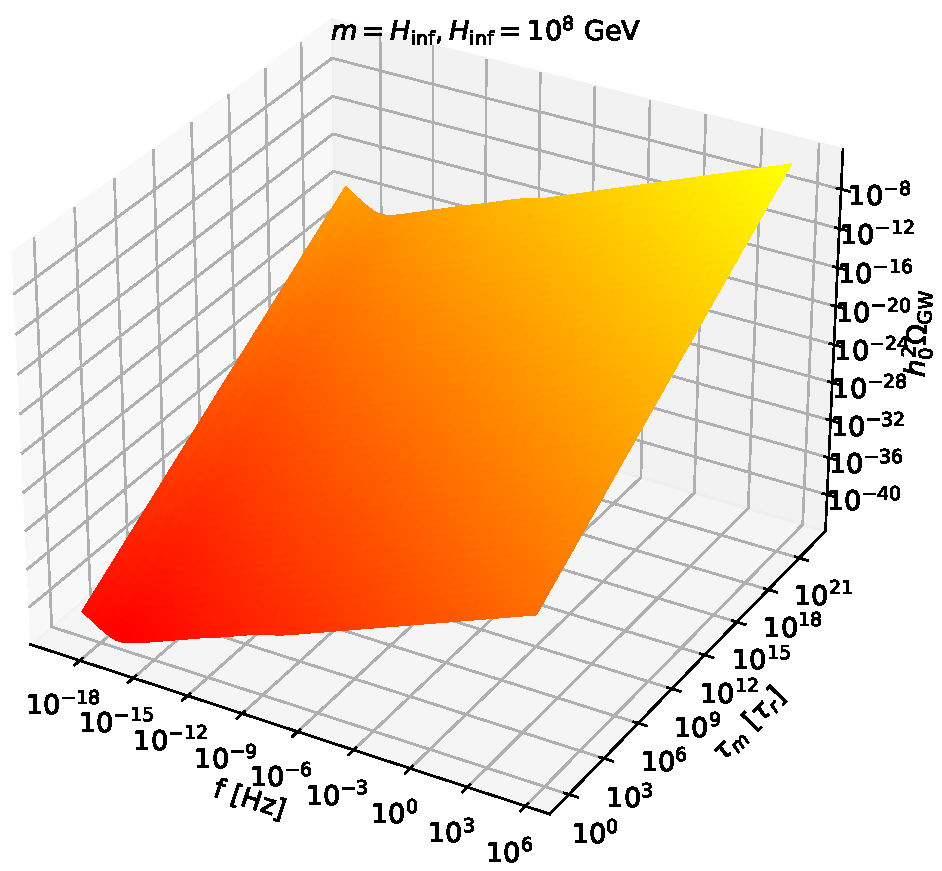
\includegraphics[width=.32\linewidth]{fig4b.pdf} 
          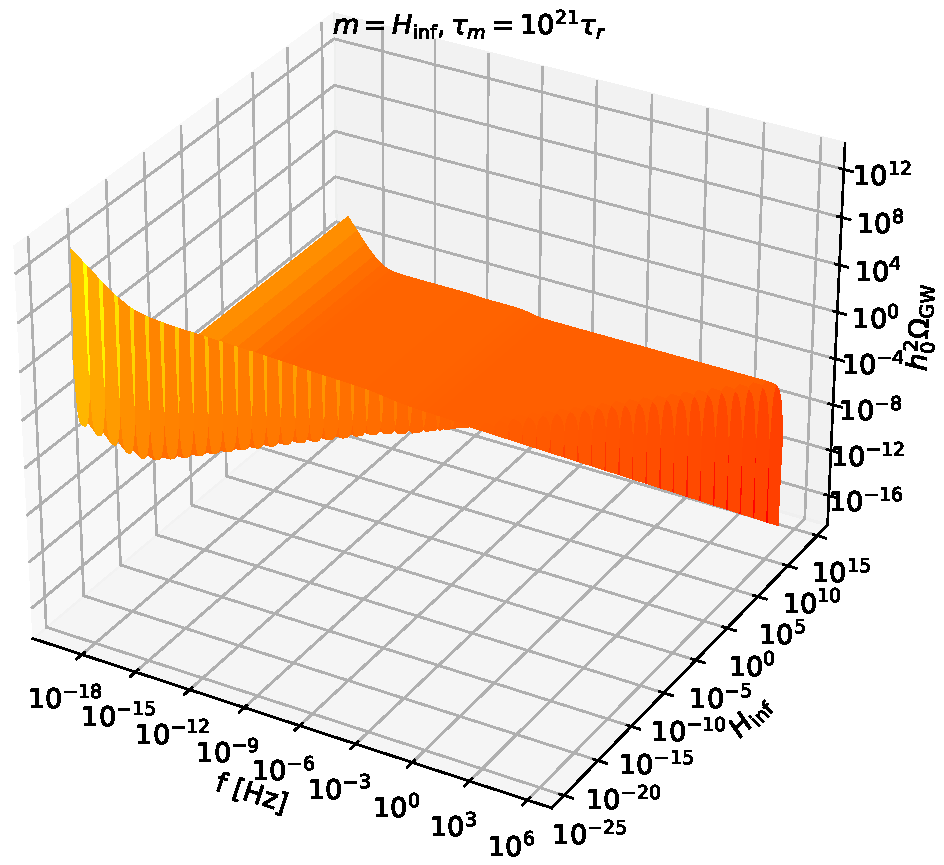
\includegraphics[width=.32\linewidth]{fig4c.pdf} 
          \label{fig:contours}
        \end{figure}
     $h_0^2\Omega_{\text{GW},0}$ as a function of $f$ and \textcolor{darksilver}{$M_{\text{GW}}$} (left), \textcolor{orange}{$\tau_m$} (middle), and \textcolor{rust}{$H_{\text{inf}}$} (right). 
  \end{tcolorbox}
  
    \begin{tcolorbox}
    \blocktitle{Results}
    
    Our values for the parameters are 
    \begin{itemize}
        \item $M_{\text{GW}} = 1.298H_{\inf}$, $H_{\inf} =  1.7 \GeV$ to stay within $1\sigma$ (\textcolor{red}{red} curve)
        \item $M_{\text{GW}} = 1.251H_{\inf}$, $H_{\inf} = 8.0 \GeV$ to stay within $2\sigma$ (\textcolor{blue}{blue} curve)
        \item $M_{\text{GW}} = 1.201H_{\inf}$, $H_{\inf} = 50. \GeV$ to stay within $3\sigma$ (\textcolor{green}{green} curve)
        \item \textcolor{purple}{purple} curve -- partially produces the signal for large $\Omega_{\text{GW}}$ and $f$
        \item \textcolor{orange}{golden} curve -- partially produces the signal for small $\Omega_{\text{GW}}$ and $f$
    \end{itemize}
   Respecting CMB, BBN bounds and reproducing the signal are mutually exclusive. If we don't respect them, we achieve good agreement with signal with a caveat: $\tau_m$ is too deep into the matter dominated era.
   \vspace{-0cm}
     \begin{figure}[t]
        \centering
          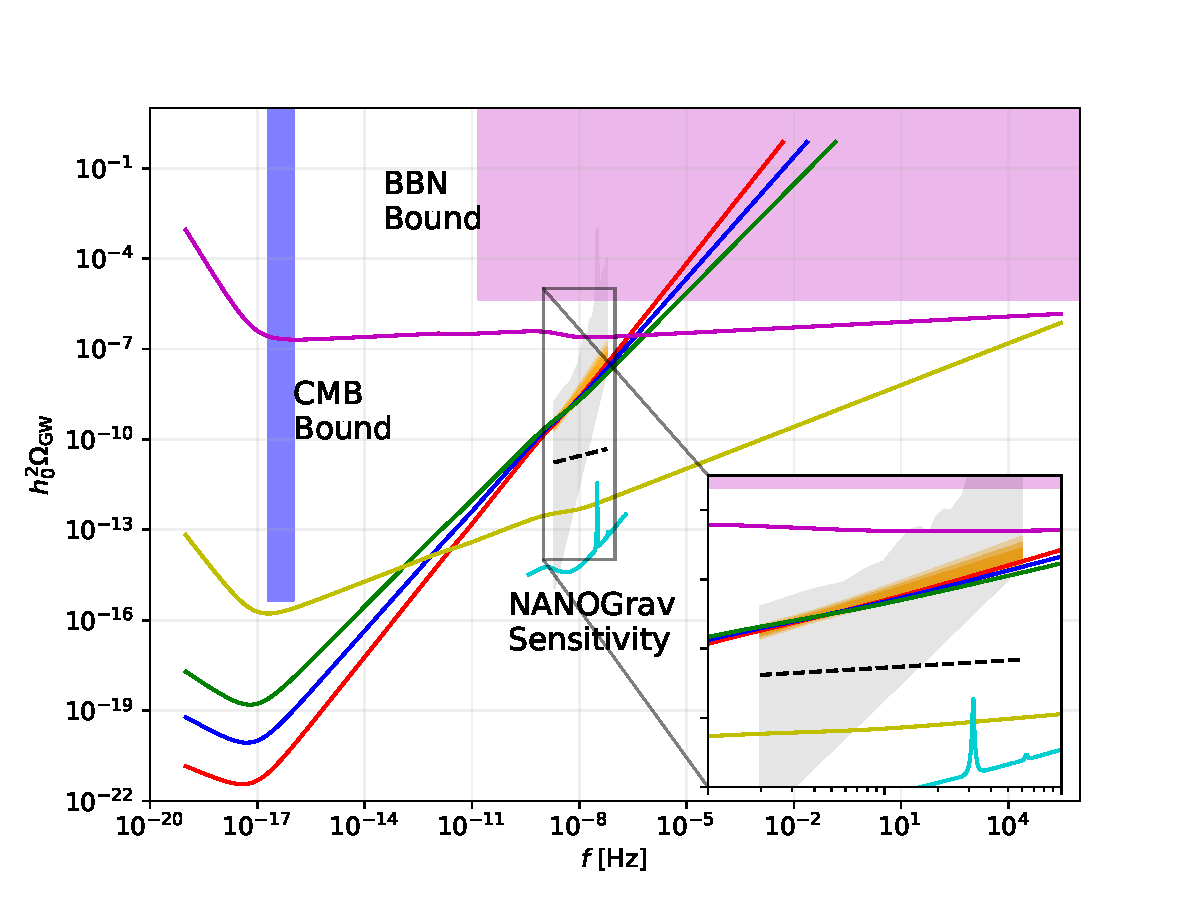
\includegraphics[width=.89\linewidth]{fig5.pdf} 
          \label{fig:gwb}
        \end{figure}
  \end{tcolorbox}
  
\end{column}

\begin{column}{0.01\textwidth}
  \begin{center}
    \textcolor{darksilver}{\rule[-1cm]{1mm}{0.8\textheight}}
  \end{center}
\end{column}

%%% column 3

\begin{column}{0.30\textwidth}
\begin{tcolorbox}
\blocktitle{Conclusions}
    \begin{itemize}
        \item Time-dependent MTMG successfully reproduces NG15
        \item BBN bound is violated for $f \gtrsim 10^{-6}$ Hz.
        \item Suppression mechanism, analogous to the damping of the energy density from the free-streaming neutrinos \cite{Durrer:1997ta}, could be introduced
        \item More complicated functions for $M_{\text{GW}}(t)$ are possible; future work can try to place constraints on the time evolution of the mass
        \item Further observations that place constraints on $H_{\text{inf}}, a_r, \tau_r$ would be able to constrain the parameters of this theory
    \end{itemize}
  \end{tcolorbox}

\begin{tcolorbox}
    \blocktitle{Source Code} 
    
    The NANOGrav 15-Year data is available at \href{https://nanograv.org/science/data}{nanograv.org/science/data}, source code to reproduce all of the figures in our paper \cite{Choi:2023tun} is available at \href{https://github.com/ChrisChoi314/constrain_mass_nanograv_15}{github.com/ChrisChoi314/constrain\_mass\_nanograv\_15} and the TeX for this poster is at \href{https://github.com/ChrisChoi314/mg_poster_aas243}{github.com/ChrisChoi314/mg\_poster\_aas243}. 
    
  \end{tcolorbox}
  
  \begin{tcolorbox}
    \blocktitle{Acknowledgements}
    
    We thank Sachiko Kuroyanagi \& Shinji Mukohyama for helpful discussions related to \cite{Fujita:2018ehq}, Axel Brandenburg, Neil J.\ Cornish, Arthur B.\ Kosowsky, \& Sayan Mandal for comments, Emma Clarke, Jeffrey S.\ Hazboun, \& William G.\ Lamb for help with plotting NG15, the organizers \& participants of the workshop \href{https://indico.cern.ch/event/1314635/overview}{``Unravelling the Universe with Pulsar Timing Arrays"}, \& Stephen Huan for the template for this poster. TK \& MG acknowledge partial support from the NASA ATP Award 80NSSC22K0825.
  \end{tcolorbox}

  \begin{tcolorbox}
    \blocktitle{Bibliography}
       \printbibliography
  \end{tcolorbox}
\end{column}

\end{columns}

\end{frame}
\end{document}